% Esta es la Plantilla UNAL en LaTeX
\documentclass[10pt,spanish,fleqn,openany,twoside,letterpaper]{book}

%Muestra los márgenes del documento para evitar Warnings
%Para activar la siguiente línea quite el simbolo % 
%\usepackage[showframe]{geometry}

%Formato de fuentes bibliográficas
%Use el estilo bibliográfico que sea pertinente según el área de estudio APA, IEEE, etc

%Usando el paquete BibLaTeX
%Cita normal con \cite[página]{} y cita con paréntesis \parencite[página]{}

% Configuración de BibLaTeX
%\usepackage[backend=biber,style=authoryear,maxcitenames=2,maxbibnames=99,giveninits=true,uniquename=false]{biblatex}
%\addbibresource{biblio.bib}

% Cambiar el idioma de las referencias bibliográficas a español
%\DefineBibliographyStrings{spanish}{%ext install latex-workshop
%  andothers = {et\addabbrvspace al\adddot},
%  andmore = {et\addabbrvspace al\adddot},
%}

% Personalizar el formato de las citas y la bibliografía
%\DeclareNameAlias{sortname}{family-given}
%\DeclareDelimFormat{multinamedelim}{\addcomma\space}
%\DeclareDelimFormat{finalnamedelim}{\addcomma\space\&\space}
%\DeclareFieldFormat{titlecase}{\MakeSentenceCase*{#1}}
%\DeclareFieldFormat[article,inbook,incollection,inproceedings,patent,thesis,unpublished]{title}{\titlecase{#1}}
%\DeclareFieldFormat{journaltitlecase}{\titlecase{#1}}
%\DeclareFieldFormat{pages}{#1}
%\DeclareFieldFormat{volume}{\mkbibbold{#1}}
%\renewbibmacro{in:}{}
%\AtEveryBibitem{\clearfield{month}}

%Usando el paquete Natbib
%Cita normal \cite[página]{} y cita con paréntesis \citep[página]{}
\usepackage{natbib}
\bibpunct{[}{]}{;}{\&}{.}{}
\bibliographystyle{dtvstyle}

%Idioma del documento
%Use main para el idioma principal del documento
\usepackage[main=spanish,english,german,french,portuguese]{babel}

% Carácteres especiales
\usepackage{fontenc}

% Evita ligadura li & fl
\usepackage{microtype}
\DisableLigatures{encoding = *, family = *}

% Otros paquetes de tablas y colores avanzados
\usepackage{amsmath,graphicx,rotating,float,multirow}
\usepackage{longtable}
\setlength{\LTcapwidth}{6in}
\usepackage[utf8]{inputenc}
\usepackage{epsfig,epic,eepic,threeparttable,amscd,here,lscape,tabularx,subfigure}
\usepackage{tabu,array}
\usepackage[rgb]{xcolor}

% Permite ver y configurar los parámetros de la página
\usepackage{layout}
%Hyperref permite ver las secciones del texto
\usepackage[hidelinks]{hyperref}

%Genera los comandos de la página de autoría
\newcommand{\studentname}{}
\newcommand{\submissiondate}{}
\newcommand{\academictitle}{}
\newcommand{\resgroupone}{}
\newcommand{\resgrouptwo}{}
\newcommand{\researchtopic}{}
\newcommand{\thesisname}{}
\newcommand{\director}{}
\newcommand{\codirector}{}
\newcommand{\issuedate}{}
\newcommand{\palabrasclave}{}
\newcommand{\keywords}{}
\newcommand{\schlusselworter}{}
\newcommand{\palavraschave}{}
\newcommand{\sede}{}
\newcommand{\department}{}
\newcommand{\faculty}{}

%Información de la tesis
%Diligenciar aquí los datos para su carga automática donde se requiera en el documento
\renewcommand{\studentname}{Andrés Felipe Vargas-Londoño}
\renewcommand{\thesisname}{CosmicWatch: The Desktop Muon Detectors, exploring gamma-ray spectroscopy}
\renewcommand{\issuedate}{2024}
\renewcommand{\submissiondate}{Fecha entrega}
\renewcommand{\director}{Prof. Luis Fernando Cristancho Mejia}
\renewcommand{\codirector}{Prof. Spencer Axani}
\renewcommand{\academictitle}{Físico}
\renewcommand{\resgroupone}{Grupo de Física Nuclear Universidad Nacional (GFNUN) }
\renewcommand{\resgrouptwo}{Axani Group (AxLab) }
\renewcommand{\researchtopic}{Espectroscopía gamma}
\renewcommand{\sede}{Sede Bogotá} 
\renewcommand{\department}{Departamento de Física}
\renewcommand{\faculty}{Facultad de Ciencias}

%Palabras clave del documento - Tener presente los Theasurus https://www.thesaurus.com/
%Disponible en 3 idiomas aunque se puede extender a francés o otro idioma
\renewcommand{\palabrasclave}{Use palabras clave que estén en Theasaurus} 
\renewcommand{\keywords}{Use keywords available in Theasaurus}
%\renewcommand{\schlusselworter}{}
%\renewcommand{\palavraschave}{}

%Formatting for headers and footers
\usepackage{fancyhdr}
\pagestyle{fancy}

\fancypagestyle{plain}

\newcommand{\RomanNumeralCaps}[1]
    {\MakeUppercase{\romannumeral #1}}

%\fancyhead[RO,LE]{Monolithic Nanocomposite Detector for LaBrAT-PET}

% Redefinir \sectionmark
\renewcommand{\sectionmark}[1]{\markright{#1}}
% Redefinir \leftmark para mostrar solo el nombre de la sección
\renewcommand{\chaptermark}[1]{\markboth{#1}{}}

% Configurar encabezado y pie de página
\fancyhead[RO]{\thepage} % Encabezado derecho en páginas impares
\fancyhead[LO]{\textbf{\leftmark}}   % Encabezado izquierdo en páginas impares
\fancyhead[RE]{\textbf{\thesisname}}   % Encabezado izquierdo en páginas pares
\fancyhead[LE]{\thepage}  % Encabezado derecho en páginas pares
\fancyfoot[C]{}            % Pie de página central vacío

\usepackage{titlesec}
% Permite personalizar los títulos de sección y de capítulos
% hang lo deja en el mismo renglón, display lo despliega
% Elimina el "Capitulo" y deja solo el número
%\titleformat{\chapter}[hang]
%  {\sffamily\Huge\bfseries}{\thechapter}{0.5cm}{\sffamily\Huge}
%\titleformat{\section}[hang]{\sffamily\LARGE}{\thesection}{0.5cm}{}
%\titleformat{\subsection}[hang]{\sffamily\Large}{\thesubsection}{0.5cm}{}
%\titleformat{\subsubsection}[hang]{\sffamily\large}{\thesubsubsection}{0.5cm}{}
%\titleformat{\paragraph}[runin]{\sffamily\normalsize}{}{}{\emph}

%Coloca anexo o apéndice en la Tabla de contenido
\usepackage[toc,page]{appendix}

% Configuración de las páginas en twoside-mode
% Permite ver y configurar los parámetros de la página
\setlength{\voffset}{-0.25in}
\setlength{\headwidth}{467pt}
\setlength{\headheight}{22pt}
\setlength{\oddsidemargin}{0pt}
\setlength{\evensidemargin}{0pt}
\setlength{\marginparwidth}{0pt}
\setlength{\marginparsep}{0pt}
\setlength{\parskip}{2em}
\setlength{\footskip}{20pt}
\setlength{\textheight}{650pt}
\setlength{\textwidth}{467pt}
\setlength{\headsep}{5pt}
\setlength{\parindent}{0pt}
\setlength{\baselineskip}{10pt plus 5pt minus 5pt}
\renewcommand{\theequation}{\thechapter-\arabic{equation}}
\renewcommand{\thefigure}{\textbf{\thechapter-\arabic{figure}}}
\renewcommand{\thetable}{\textbf{\thechapter-\arabic{table}}}


%Define la distancia de la primera linea de un parrafo a la margen
\parindent0cm 

%Espacio entre lineas
\renewcommand{\baselinestretch}{1}

%Para rotar texto, objetos y tablas seite.
\usepackage{rotating}

%Permite incluir mecanismos y reacciones químicas
\usepackage{tikz}
\usepackage{chemformula}
\usepackage{chemfig}

\usetikzlibrary{calc,arrows.meta}% per right to e left to
\tikzset{
myedge/.style={->, -{Latex[#1]}}
}

%Fuente de la presentación Ancizar Sans UNAL
%Para usar este compilado en Overleaf se debe usar el compilador XeLaTeX o LuaLaTeX!!
%Menu -> Compiler -> XeLaTeX o LuaLaTeX
%La siguiente línea debe comentarse si desea compilar con pdfLaTeX
%\RequireXeTeX


% Definición de la fuente Ancizar Sans
\newif\ifxetexorluatex

\ifxetexorluatex
  \usepackage{fontspec}
  \usefonttheme{serif}
  \setmainfont{AncizarSans}[Path=./AncizarSans/,Scale=1,Extension=.otf,UprightFont=*-Regular,BoldFont=*-Bold,ItalicFont=*-Italic,BoldItalicFont=*-BoldItalic]
\else
  % Si se compila con pdfLaTeX, cargar la fuente apropiada aquí
  \usepackage[T1]{fontenc}
\fi
% Metadatos del documento
\AtBeginDocument{%
	\hypersetup{
		pdfborder={0 0 0},
		pdfauthor={\studentname},
		pdfsubject={\thesisname}, 
		pdfcreator={\studentname},
		pdfproducer={\studentname},
	}
}

%Carga el simbolo de grado y el de Angstrom
\newcommand{\angstrom}{\textup{\AA}}
\newcommand{\grad}{$^{\circ}$}

%Inicio del documento, no olvide la etiqueta de cierre al final \end{document}
\begin{document}

%Nombres y formatos de títulos, tablas y figuras
%Use \sffamily para dejar con letra Sans Serif, sin etiqueta queda LaTeX clásico
\renewcommand{\listfigurename}{List of Figures}
\renewcommand{\listtablename}{List of Tables}
\renewcommand{\contentsname}{Table of contents}
\renewcommand{\chaptername}{Chapter}
%\renewcommand{\tablename}{\scriptsize \centering \textbf{Tabla}}
%\renewcommand{\figurename}{\scriptsize \centering \textbf{Figura}}
\renewcommand{\appendixname}{Appendix}

%Cambia el nombre de la sección de referencias
\renewcommand{\bibname}{Bibliography}

%Páginas de Presentación del documento - No modificar esto se hace automáticamente
{\newpage
\thispagestyle{empty}
\begin{center}
\begin{figure}
\centering

\epsfig{file=figures/EscudoUN2016,scale=1}%
\end{figure}
\vspace{2.5cm}
\textbf{\Huge \thesisname} \\ 
\vspace{2.5cm}
\textbf{\Large \studentname} \\
\vspace{5.0cm}
\small Universidad Nacional de Colombia \\
\faculty \\
\department \\
\sede, Colombia\\
\issuedate
\newpage 
\thispagestyle{empty}
\vspace{2.5cm}
\textbf{\Huge \thesisname} \\
\vspace{2.5cm}
\textbf{\Large \studentname} \\
\vspace{2.5cm}
\small Tesis presentada como requisito parcial para optar por el título de: \\
{\bfseries \academictitle}\\
\vspace{2.5cm}
Director(a): \\
\director \\
Codirector(a): \\
\codirector \\
\vspace{2.5cm}
Línea de investigación: \\ 
\researchtopic\\
Grupo de investigación: \\
\resgroupone \\
\resgrouptwo \\
\vspace{2.0cm} 
Universidad Nacional de Colombia \\
\faculty \\
\department \\
\issuedate
\end{center}

% Dedicatorias
\newpage
\thispagestyle{empty}
\begin{flushright}
\begin{minipage}{12.5cm}
\noindent
\\[10em]
%Modificar la cita que se quiere agregar
{\Large Cita 01.}
\\[3em]
Autor
\\ \textit{Fuente}
\\[10em]
%Para anular la adición de una segunda cita anule las siguientes lineas desde acá mediante comentario (%)
{\Large \textit{Wenn du es nicht einfach erkl\"{a}ren kannst, hast du es nicht genug verstanden} - Si no eres capaz de explicar algo claramente, es que aún no lo has entendido lo suficiente.}
\\[3em]
Albert Einstein
%Hasta acá!
\end{minipage}
\end{flushright} 

% Declaracíon de originalidad del texto y del contenido
% No modificar, se hace automáticamente con los comandos ya definidos
\newpage
\chapter*{Declaración}\chaptermark{Declaración}
\par Me permito afirmar que he realizado ésta tesis de manera autónoma y con la única ayuda de los medios permitidos y no diferentes a los mencionados el presente texto. Todos los pasajes que se han tomado de manera textual o figurativa de textos publicados y no publicados, los he reconocido en el presente trabajo. Ninguna parte del presente trabajo se ha empleado en ningún otro tipo de tesis. 
\\[1em]
\sede., \submissiondate
\\[6em]
\rule{6cm}{0.5pt}\\
\studentname
}

%Páginas preámbulo, listado de figuras, tablas y tabla de contenido
{\pagestyle{plain} \pagenumbering{roman}
\setlength{\parskip}{1mm}
\chapter*{Acknowledgments}\chaptermark{Acknowledgments}
\addcontentsline{toc}{chapter}{Acknowledgments}%

This goes to my family, especially to my parents, for providing me with the most sincere and unconditional support I could have ever received. To every friend who stood there when things felt overwhelming and gave me the courage to keep going. Also to every professor and mentor who generously shared their knowledge and advice.
\\

A special thanks goes to Professor Fernando Cristancho for introducing me to an extremely nurturing working environment, filled with people without whom this could never have come to be. I am also deeply grateful to Professor Spencer N. Axani, for opening the doors to not only his group but also to immensely rewarding experiences and knowledge I will carry with me forever.
\\

Last but not least I want to thank me for believing in me, I want to thank me for doing all this hard work, for never quitting and for being me at all times.   
\chapter*{Listado de símbolos y abreviaturas}\chaptermark{Listado de símbolos y abreviaturas}
\addcontentsline{toc}{chapter}{Listado de símbolos y abreviaturas}
\newpage
\chapter*{Resumen}\chaptermark{Resumen}
\addcontentsline{toc}{chapter}{Resumen}%
\textbf{\Huge \ \strut CosmicWatch: Los Detectores de Muones de Escritorio, explorando la espectroscopia gamma \strut} %strut keeps interline spacing consistent
\vspace{.5cm}
\par El presente trabajo se concentra en el mejoramiento de CosmicWatch: Los Detectores de Escritorio de Muones, con el objetivo de obtener una resolución en energías suficiente para realizar espectroscopía gamma. Dadas ciertas limitaciones actuales en la electrónica, como tiempo muerto y baja rata de conteo, junto con la baja resolución de los centellatores plásticos usados hasta ahora, este trabajo explora entonces el uso de una RaspberryPi Pico y un cristal centellador basado en Lutecio y dopado con Cerio (LYSO:Ce), logrando resolución en energías de $13.5\%$ para 511 \unit{\kilo\eV} al medir con un osciloscopio Rohde\&Schwarz RTO6 y $28.3\%$ con modulos NIM.
\\[2cm]
\textbf{Palabras clave:} \palabrasclave

\newpage 
\chapter*{Abstract}\chaptermark{Abstract}
\addcontentsline{toc}{chapter}{Abstract}%
\textbf{\Huge \ \strut CosmicWatch: The Desktop Muon Detectors, exploring gamma-ray spectroscopy \strut} %strut keeps interline spacing consistent
\vspace{.5cm}
\par The present work focuses on the improvement of CosmicWatch: The Desktop Muon Detectors, with the goal of achieving sufficient energy resolution to allow for gamma spectroscopy. Due to current limitations in the electronics, such as dead time and small sample rate, in addition to the low energy resolution of previously used plastic scintillators, this work explores the use of a RaspberryPi Pico together with a Cerium-doped Lutetium-based scintillation crystal (LYSO:Ce), achieving energy resolutions of $13.5\%$ at 511 \unit{\kilo\eV} while sampling data with a Rohde\&Schwarz RTO6 oscilloscope and $28.3\%$ with NIM modules.
\\[2cm]
\textbf{Keywords:} \keywords

%\newpage 
%\chapter*{\sffamily Zusammenfassung}
%\addcontentsline{toc}{chapter}{Zusammenfassung}%
%\par Zusammenfassung texte.
%\par 
%\\[2cm]
%\textbf{Schlüsselwörter:} \schlusselworter
\tableofcontents 
\addcontentsline{toc}{chapter}{Table of contents}
\listoffigures 
\addcontentsline{toc}{chapter}{List of Figures}
\listoftables 
\addcontentsline{toc}{chapter}{List of Tables}
\clearpage
}

{\pagenumbering{arabic}
\setlength{\parskip}{\baselineskip}
%Incluir secciones del documento de aqui en adelante
%Use \include para incluir desde una página nueva e \input para incluir sin salto de página
\chapter{Introduction}

CosmicWatch: The Desktop Muon Detectors \cite{axani2019physics}, is a self-contained, low-cost, and easy-to-build particle detector for students, scientists, and cosmic-ray enthusiasts. It aims to make particle detection interactive and available to anyone interested in learning about the electronics and physics involved in this area of expertise. With this in mind, the detector design prioritizes the user experience across the board, from its construction to data acquisition and processing. It uses a silicon photomultiplier (SiPM) to collect light emitted by a plastic scintillator after a charged particle, like a cosmic-ray muon, deposits some of its energy in it. This project aims to further expand the capabilities of CosmicWatch by exploiting the already existing electronics and implementing the necessary features to transform the detector into a portable gamma-ray spectrometer

So far, previous iterations of CosmicWatch have not focused on the energy deposition of particles in the detector due to the poor resolution of the scintillating materials used, generally plastic scintillators such as BC-400/404. The current software and hardware speeds also represent a limiting factor, introducing dead time and therefore decreasing the sample rate. By switching to a Cerium-doped Lutetium-based scintillation crystal (LYSO:Ce), testing new electronics, and implementing better programming paradigms, this work thus aims to further explore and expand the capabilities of CosmicWatch, hoping to one day provide a self-contained, low-cost, and easy-to-build particle detector suited for gamma-ray spectroscopy.
\chapter{Goals}
\chapter{Electronics}
\label{chap:Electronics}

CosmicWatches have to be mainly low-cost and easy to build. In order to achieve this, the components selected for the construction have been carefully curated to make sure these restrictions were met. This however might be greatly responsible for some of the odd features found while testing the detector, like the lack of linearity and fluctuations in amplification and peak-detected values of seemingly equal input signals. The full KiCad project can be found in the GitHub repository: \href{https://github.com/anvargasl/CosmicWatch-gamma-spectroscopy-PCB}{CosmicWatch-gamma-spectroscopy-PCB}. The component numbers shown in this chapter are the ones that would have to be placed on the PCB in order to recreate the example schematics.

\begin{figure}[H]
    \centering
    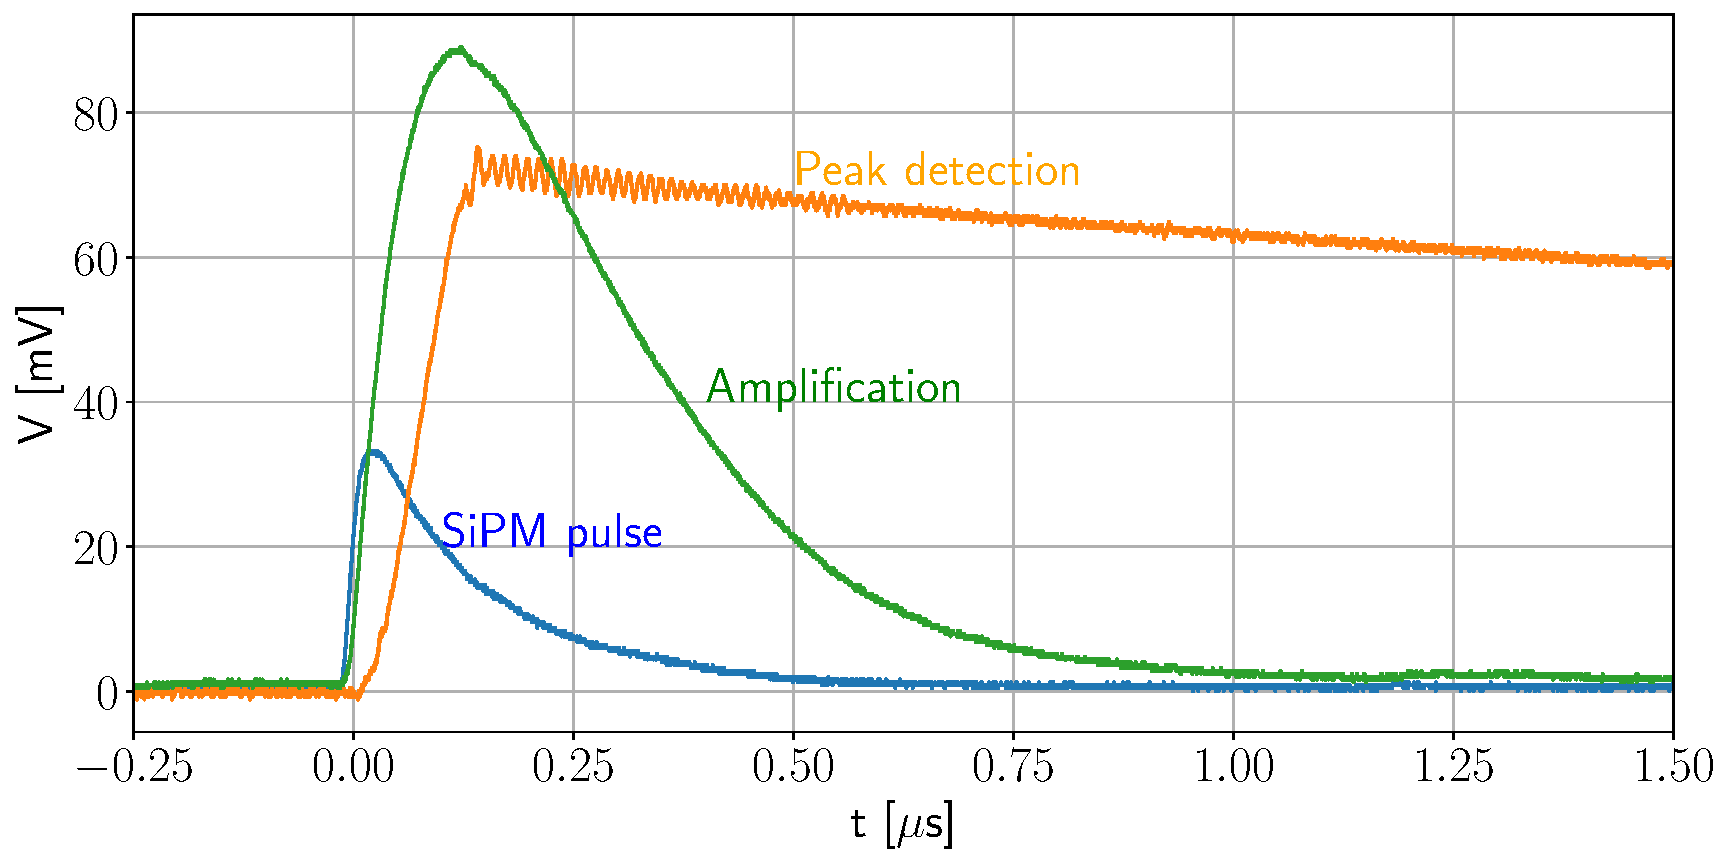
\includegraphics[width=0.8\textwidth]{Electronics/CW-signals.pdf}
    \caption{Signal processing inside the detector.}
    \label{fig:signal_processing}
\end{figure}

\section{Amplifier}

\begin{figure}[H]
    \centering
    \begin{circuitikz}[scale=0.7]
        \draw
        (0,0) node[op amp, noinv input up, font=\small] (opamp) {$U6$}
        (opamp.up) --++(0,0.5) node[vcc]{5\,\textnormal{V}}
        (opamp.down) --++(0,-0.5) node[vee]{-5\,\textnormal{V}}
        (opamp.+) node[left]{$V_{in}$}
        (opamp.-) node[left]{} to[short] ++(0, -3) coordinate(R4_R)
        to[R, l_=$R_4$] ++(-3, 0) node[ground]{}
        (R4_R) to[R, l_=$R_6$] ++(2.7, 0)
        %to[short] ++(0.1, 0) -|(opamp.out) to[short] ++(1, 0) node[ocirc, label={[yshift=0.3]$V_{out}$}]{}
        to[short] ++(0.1, 0) -|(opamp.out) to[short,-*] ++(1,0) node[above]{$V_{out}$};
        %to[short] ++(1, 0) node[ocirc, label=above:$V_{out}$]{};

        %Nodes
        %\node[shift={(0,+1.5)}] at (opamp) {U6 HLM6658};
    \end{circuitikz}
    \caption{Amplifier circuit schematic. An LT1807 op-amp is used for this and the peak detection stage.}
    \label{circ:amplifier}
\end{figure}

The processing of a pulse coming out of the SiPM has to go through two main stages, amplification and peak detection, Fig. \ref{fig:signal_processing} showcases these stages. The brightest SiPM pulses seen so far do not exceed 200 mV, which covers a very small portion of the ADC range on the RP Pico (0-3.3 V \cite[p.~18]{datasheet2024rp2040}). Amplification of the signal therefore allows for better resolution.

An op-amp on its own amplifies the voltage difference between the non-inverting (pin $+$) and inverting (pin $-$) inputs by its internal gain $A_{int}$, having then $V_{out}=A_{int}(V_+ - V_-)$. In this case, however, we are interested in controlling the gain of the circuit and therefore the amplification. In order to achieve this we introduce a feedback loop in the op-amp through $R4$ and $R6$, which controls how much of the output voltage is fed back into the op-amp. The theoretical amplification is therefore given by $V_{out}=(1+R6/R4)V_{in}$. A simple schematic showcasing the component arrangement is shown in Fig. \ref{circ:amplifier}.

\section{Peak Detector}

Since the LYSO crystal is so fast (36 ns of decay time \cite{Luxium_LYSO}) the ADC sample rate and response time of the Pico both play an important role in the number of events that the detector will accurately acquire. It is therefore necessary to hold the voltage of the amplified pulse in order to increase the chances of reading the actual value of the incoming signal. This is the task of the peak detector, to widen the time window in which we can sample the ADC and get a correct reading.

The idea behind the peak detector is to store charge in a capacitor ($C_{25}$) through a diode ($D_3$), retaining the highest voltage the input signal has reached. A diode is placed before the capacitor so that once the signal's voltage goes below the peak voltage, the diode will be reverse biased, therefore preventing current from flowing while maintaining the voltage on the capacitor.

In order to measure the voltage in the capacitor, a discharging resistor has to be added ($R_{15}/R_{19}$). The time it takes the capacitor to discharge is given by $t=RC$. Although for example in the case of CosmicWatch-V2's peak detector, the values of $R_{14}$ and $R_{24}$ also play a role in the discharging time, which has proved not to be as trivial as calculating the equivalent resistance $R_t$ of all three and simply take $t=R_tC$.

The schematic and PCB shown in the repository \href{https://github.com/anvargasl/CosmicWatch-gamma-spectroscopy-PCB}{CosmicWatch-gamma-spectroscopy-PCB}, include the connections and footprints necessary to place the components that make the designs illustrated in Subsections \labelcref{sec:basic,sec:pd_V2,sec:basic_buffer,sec:nuclear_phoenix}. Different results were found while testing these peak detector setups.

\subsection{Basic Peak Detector}\label{sec:basic}

\begin{figure}[H]
    \centering
    \begin{circuitikz}[scale=0.7]
        %\draw [help lines] (-4,0) grid (5,-4);
        \draw (0,0) node[op amp, noinv input up, font=\small] (opamp) {$U6$}
        (opamp.up) --++(0,0.5) node[vcc]{5\,\textnormal{V}}
        (opamp.down) --++(0,-0.5) node[vee]{-5\,\textnormal{V}}
        (opamp.+) node[left]{$V_{in}$}
        (opamp.out) node[]{} to[sD, l_=$D_3$] (6, 0) coordinate (D3_r)
        (opamp.-) node[left]{} to[short] ++(0, -2.5) coordinate (R24_l)
        (R24_l) to[R, l^=$R_{24}$, resistors/scale=0.8] (D3_r |- , |- R24_l) coordinate (R24_r)
        (D3_r) -- (R24_r)
        (D3_r) -- ++(1,0) coordinate (C25_u)
        (C25_u) to[C, l=$C_{25}$] ++(0,-2) node[ground]{}
        (C25_u) -- ++(2,0) to[R, l=$R_{15}$, resistors/scale=0.8] ++(0,-2) node[ground]{};
        %\draw (A |- 52,3)(D3_r) -- (R24_r);
        % to[short] ++(-0.1, 0) -|(R24_r)
    \end{circuitikz}
    \caption{Basic peak detector design.}
    \label{circ:basic_pd}
\end{figure}

Assuming ideal conditions, a diode is enough to retain the highest input voltage reached. Semiconductor diodes however don't behave ideally, they introduce a voltage drop that will keep the voltage stored in $C_{25}$ at a lower potential than that of $V_{in}$. In order to prevent this, an op-amp $(U_6)$\footnote{Currently the only op-amp that has behaved reasonably well is the LT1807 by Analog Devices Inc. The LMH6658  by Texas Instruments seems to have trouble driving even small capacitors.} is placed before the diode. In the configuration shown in Fig. \ref{circ:basic_pd}, the opamp will try to output the necessary current to equilibrate the inverting input voltage (pin $-$) to what it sees in the non-inverting input (pin $+$), to achieve this $U_6$ has to go one diode drop above $V_{in}$.

\subsection{Preventing negative saturation}\label{sec:pd_V2}

\begin{figure}[H]
    \centering
    \begin{circuitikz}[scale=0.7]
        %\draw [help lines] (-4,0) grid (5,-4);
        \draw (0,0) node[op amp, noinv input up, font=\small] (opamp) {$U_6$}
        (opamp.up) --++(0,0.5) node[vcc]{5\,\textnormal{V}}
        (opamp.down) --++(0,-0.5) node[vee]{-5\,\textnormal{V}}
        (opamp.+) node[left]{$V_{in}$}
        (opamp.out) -- ++(1,0) coordinate(oa_out) to[sD, l_=$D_3$] (6, 0) coordinate (D3_r)
        (opamp.-) -- ++(0, -2.7) coordinate (ver_1) -- ++(1, 0) coordinate(D5_l)
        (ver_1) to[R, l_=$R_{14}$, resistors/scale=0.8] ++(-2,0) node[ground]{} 
        (D5_l) to[sD, l_=$D_5$] (oa_out |- , |- D5_l) coordinate (D5_r)
        (oa_out) -- (D5_r)
        (D5_l) -- ++(0,-1.7) coordinate (R24_l)
        (R24_l) to[R, l^=$R_{24}$, resistors/scale=0.8] (D3_r |- , |- R24_l) coordinate (R24_r)
        (D3_r) -- (R24_r)
        (D3_r) -- ++(1,0) coordinate (C25_u)
        (C25_u) to[C, l=$C_{25}$] ++(0,-2) node[ground]{}
        (C25_u) -- ++(2,0) to[R, l=$R_{15}$, resistors/scale=0.8] ++(0,-2) node[ground]{};
    \end{circuitikz}
    \caption{Basic peak detector design, a second diode is added in order to prevent the op-amp from entering a negative saturation loop.}
    \label{circ:pd_V2}
\end{figure}

In the basic peak detector, once the signal voltage goes below the peak voltage, $D_3$ will be reverse biased and the inverting input of the opamp will see a higher voltage than the non-inverting input, this will force $U_6$ to go into negative saturation by driving the output voltage as low as it can in order to match both inputs. Once the signal gets close to the stored voltage in $C_25$, the op-amp will have to get out of the negative saturation, this will take some time which depends on the slew rate of the opamp and therefore limits the operating frequency range of the circuit.

In order to avoid negative saturation $D_5$ is added, along with an outer feedback loop through $R_{24}$. In this case, once the input signal goes below the stored voltage, $D_5$ will be forward biased, allowing for a new feedback loop that decreases the op-amp's negative saturation time.


\subsection{Basic Peak Detector + Buffer}\label{sec:basic_buffer}

\begin{figure}[H]
    \centering
    \begin{circuitikz}[scale=0.7]
        %\draw [help lines] (-4,0) grid (5,-4);
        \draw (0,0) node[op amp, noinv input up, font=\small] (opamp) {$U_6$}
        (opamp.up) --++(0,0.5) node[vcc]{5\,\textnormal{V}}
        (opamp.down) --++(0,-0.5) node[vee]{-5\,\textnormal{V}}
        (opamp.+) node[left]{$V_{in}$}
        (opamp.out) -- ++(1,0) coordinate(oa_out) to[sD, l_=$D_3$] (6, 0) coordinate (D3_r)
        (opamp.-) -- ++(0, -2.7) coordinate (ver_1) -- ++(1, 0) coordinate(D5_l)
        (ver_1) to[R, l_=$R_{14}$, resistors/scale=0.8] ++(-2,0) node[ground]{} 
        (D5_l) to[sD, l_=$D_5$] (oa_out |- , |- D5_l) coordinate (D5_r)
        (oa_out) -- (D5_r)
        (D5_l) -- ++(0,-1.7) coordinate (R24_l)
        (D3_r) -- ++(1,0) coordinate (C25_u)
        (C25_u) to[C, l=$C_{25}$] ++(0,-2) node[ground]{}
        (C25_u) -- ++(2,0) coordinate (buffer_l)
        (buffer_l) node[op amp, noinv input up, font=\small, anchor=+] (buffer) {$U_7$}
        (buffer.-) coordinate (buffer_-)
        (buffer.out) coordinate (buffer_out)
        (buffer_-) -- (buffer_- |-, |- R24_l) coordinate (R24_r)
        (R24_l) to[R, l^=$R_{24}$, resistors/scale=0.8] (R24_r)
        (R24_r) -- (buffer_out |-, |- R24_r) -- (buffer_out)
        (buffer_out) to[short, -*] ++(1,0);
        %(D3_r) -- (R24_r);
        %(C25_u) -- ++(2,0) to[R, l=$R_{15}$, resistors/scale=0.8] ++(0,-2) node[ground]{};
    \end{circuitikz}
    \caption{Basic peak detector design, Adding a buffer to prevent discharging of the capacitor through the resistor and instead through any load in the circuit, in this case $R_{29}$.}
    \label{circ:pd_buffer}
\end{figure}

This design follows the same principles as the one shown in the previous subsection. However, in this case, a buffer is added to introduce high impedance and prevent the capacitor from discharging through the resistor and instead through any load that may be applied after the circuit.

\subsection{Nuclear Phoenix}\label{sec:nuclear_phoenix}

\begin{figure}[H]
    \centering
    \begin{circuitikz}[scale=0.7]
        %\draw [help lines] (-4,0) grid (5,-4);
        \draw (0,0) node[op amp, noinv input up, font=\small] (opamp) {$U_6$}
        (opamp.up) --++(0,0.5) node[vcc]{5\,\textnormal{V}}
        (opamp.down) --++(0,-0.5) node[vee]{-5\,\textnormal{V}}
        (opamp.+) node[left]{$V_{in}$}
        (opamp.out) coordinate(oa_out) to[sD, l_=$D_5$] ++(2, 0) coordinate (D5_r)
        (D5_r) to[sD, l_=$D_3$] ++(2, 0) coordinate (D3_r)
        (D5_r) -- ++(0,-4) coordinate (R30_l)
        (D3_r) -- ++(3,0) coordinate (C25_u)
        (C25_u) to[C, l=$C_{25}$] ++(0,-2) node[ground]{}
        (C25_u) -- ++(2,0) coordinate (buffer_l)
        (opamp.-) coordinate (oa_-)
        (oa_-) -- ++(-1.5, 0) -- ++(0, 4) coordinate(aux1)
        (aux1) -- (D3_r |-, |- aux1) -- (D3_r)
        (buffer_l) node[op amp, noinv input up, font=\small, anchor=+] (buffer) {$U_7$}
        (buffer.-) coordinate (buffer_-)
        (buffer.out) coordinate (buffer_out)
        (buffer_-) -- (buffer_- |-, |- R30_l) coordinate (R30_r)
        (R30_l) to[R, l_=$R_{30}$, resistors/scale=0.8] (R30_r)
        (R30_r) -- (buffer_out |-, |- R30_r) -- (buffer_out)
        (buffer_out) to[short, -*] ++(1,0);
        %(D3_r) -- (R24_r);
        %(C25_u) -- ++(2,0) to[R, l=$R_{15}$, resistors/scale=0.8] ++(0,-2) node[ground]{};
    \end{circuitikz}
    \caption{Nuclear Phoenix peak-detector design. Taken from \cite{Nucelar_phoenix}.}
    \label{circ:pd_np}
\end{figure}

NuclearPhoenix is a physics student who has developed a gamma detector that also utilizes a Raspberry Pi Pico and a Silicon photomultiplier, his schematics also include a peak detection circuit which is shown in Fig. \ref{circ:pd_np}, his project can be found in \href{https://nuclearphoenix.xyz/hardware/ogd/}{Open Gamma Detector}. This design aims to prevent leakage current across $D_3$, this discharges the capacitor at a faster rate than intended once the peak voltage has been reached. In this case, $R_30$ is feeding back the peak voltage value to $D_3$, therefore creating a 0 V difference across the diode, preventing any leakage current from flowing out of $C_{25}$ and into the output of the op-amp.

\section{Trigger}

\begin{figure}[H]
    \centering
    \begin{circuitikz}[scale=0.7]
        %\draw [help lines] (-4,0) grid (5,-4);
        \draw (0,0) node[op amp, noinv input up, font=\small] (opamp) {$U_6$}
        (opamp.up) --++(0,0.5) node[vcc]{5\,\textnormal{V}}
        (opamp.down) --++(0,-0.5) node[vee]{-5\,\textnormal{V}}
        (opamp.out) --++(1,0) node[above]{$V_{out}$}
        (opamp.+) node[left]{$V_{in}$}
        (opamp.-) --++(-2.5,0)  coordinate (oa_-)
        (oa_-) to[R, l^=$R_{16}$, resistors/scale=0.8] ++(0,2) to[R, l^=$R_{22}$, resistors/scale=0.8] ++(0,2) node[vcc]{5\,\textnormal{V}}
        (oa_-) to[R, l_=$R_{18}$, resistors/scale=0.8] ++(0,-2) node[ground]{};

        %Nodes
        \node[shift={(-0.3,-0.3)}] at (opamp.-) {$V_{REF}$};
    \end{circuitikz}
    \caption{Trigger circuit.}
    \label{circ:trigger}
\end{figure}

In this case, a voltage divider is used to force a positive saturation in the op-amp once the amplified signal reaches a threshold voltage, generating a "digital 1"\: that can be used to trigger the detector. The threshold, or $V_{REF}$ as noted in Fig. \ref{circ:trigger}, is given by equation \eqref{eq:v_ref}.

\begin{equation}
    V_{REF}=\frac{R_{18}}{R_{22}+R_{16}+R_{18}} V_{cc} \label{eq:v_ref}
\end{equation}

%add code as appendix
\section{Microcontroller}

\section{DC to DC booster}

\begin{figure}[H]
    \centering
    \begin{circuitikz}
        % U1 NE555
        \draw [thick] (0,0) coordinate (u1) rectangle ++(2,3); % shape
        \draw [pin] (u1) ++(1, 3.8)
            node[]{$U_1$};
        \draw [pin] (u1) ++(1, 3.3)
            node[]{MAX5026};
        %-----------Left side-----------%
        \draw [pin] (u1) ++ (0,2.5) coordinate (u1 pgnd)
            node[right, font=\scriptsize]{PGND}
            node[above left]{1}; % CON
        \draw [pin] (u1) ++ (0,1.5) coordinate (u1 gnd)
            node[right, font=\scriptsize]{GND}
            node[above left]{2}; % TRI
        \draw [pin] (u1) ++ (0,0.5) coordinate (u1 fb)
            node[right, font=\scriptsize]{FB}
            node[above left]{3}; % THR
        
        %-----------Right side-----------%
        \draw [pin] (u1) ++ (2,2.5) coordinate (u1 lx)
            node[left, font=\scriptsize]{LX}
            node[above right]{6}; % OUT
        \draw [pin] (u1) ++ (2,1.5) coordinate (u1 vcc)
            node[left, font=\scriptsize]{VCC}
            node[above right]{5}; % OUT
        \draw [pin] (u1) ++ (2,0.5) coordinate (u1 shdn)
            node[left, font=\scriptsize]{SHDN}
            node[above right]{4}; % OUT
        %\draw (u1) ++ (2,0)
        %    node[right]{\ctikzlabel{$U_1$}{NE555}}; % NE555P
        
        % U1 NE555 Pins
        \draw (u1 pgnd) -- ++ (-1,0) node[ground]{}; % PGND

        \draw (u1 gnd) -- ++ (-1,0) node[ground]{}; % GND

        \draw (u1 fb) -- ++ (-2,0) coordinate(r10 u) to[R, l_=$R_{10}$, resistors/scale=0.8] ++(0,-2) node[ground]{}
        (r10 u) to[R, l^=$R_{2}$, resistors/scale=0.8] ++(0,2) -- ++(0,2) -- ++(7,0) coordinate(d4 r)
        (d4 r) --++(2,0) coordinate(c3 u) to[R, l^=$R_{25}$, resistors/scale=0.8] ++(2,0) coordinate (c4 u)
        (c3 u) to[C, l_=$C_{3}$, resistors/scale=0.8] ++(0,-2)  node[ground]{}
        (c4 u) to[C, l_=$C_{4}$, resistors/scale=0.8] ++(0,-2)  node[ground]{}
        (c4 u) --++(1,0) node[vcc]{\textnormal{HV}}; % FB

        \draw (u1 lx) -- ++ (1,0) coordinate(d4 l)
        (d4 l) -- ++(0,1) to[sD, l^=$D_3$] ($(d4 r) + (0,-1)$) -- (d4 r)
        (d4 l) to[american inductor, l_=$L_1$] ($(d4 r) + (0,-2)$) coordinate(l1 r); % LX

        \draw (u1 vcc) -- ++ (1,0) to[short, -*] ++(0,-1); % VCC

        \draw (u1 shdn) --++(2,0) coordinate(c7 u) --++(1,0) coordinate (c2 u) --(l1 r)
        (c7 u) to[C, l_=$C_{7}$, resistors/scale=0.8] ++(0,-2) node[ground]{}
        (c2 u) to[C, l=$C_{2}$, resistors/scale=0.8] ++(0,-2) node[ground]{}
        (c2 u) --++(1,0) node[vcc]{5\,\textnormal{V}}; % SHDN
    \end{circuitikz}
    \caption{DC to DC booster circuit. Careful considerations have to be made when placing the MAX5026 IC in order to reduce noise on the power line. It is advised to have a look at the datasheet in \cite{AnalogDevices_DC_DC}, section "Applications Information".}
    \label{circ:booster}
\end{figure}

Acording to Onsemi \cite{Onsemi_SiPM}, the operaing voltage of a MicroFJ-300XX-TSV SiPM is 25.2-30.7 V. It is then necessary to boost $V_{cc}$ to the operating range of the SiPM, noted as HV in Fig. \ref{circ:booster}. In order to achive this, a MAX5026 PWM Step-Up DC-DC Converter is used \cite{AnalogDevices_DC_DC}, which has a user-adjustable output voltage of up to 36 V using external feedback resistors.

In the circuit shown in Fig. \ref{circ:booster}, $R_{10}$ and $R_2$ determine the output voltage HV. According to \cite{AnalogDevices_DC_DC}, equation \eqref{eq:booster_fb_resistance} allows to calculate the Value of $R_{10}$ given a desired output voltage HV and a value of $R_2$ between 5 and 50 \unit{\kilo\ohm}.

\begin{equation}
    R_{10} = R_2\left(\frac{\text{HV}}{V_{REF}}-1\right) \label{eq:booster_fb_resistance}
\end{equation}

\section{Single photons}
\chapter{Gamma Spectroscopy}

\section{Generalities}

\subsection{Gamma Sources}

\subsubsection{Beta decay}

\subsubsection{Electronic Capture}

\subsubsection{Internal Conversion}

\section{Scintillation}

%Inicio del apéndice o anexos
\begin{appendix}
\chapter{Appendix 1}%
\end{appendix}

%Permite visualizar la bibliografía en la tabla de contenido
\addcontentsline{toc}{chapter}{References} %Literatura Citada

\let\OLDthebibliography=\thebibliography
\def\thebibliography#1{\OLDthebibliography{#1}}
{\scriptsize
\pagestyle{plain}
% Nombre del documento donde se almacenan las referencias
\bibliography{Referencias}
\nocite{*}
\cleardoublepage
}
}

\end{document}